%UNIT 10: SPRING MASS SYSTEM AND LINEAR SYSTEMS
%%%%%%%%%%%%%%%%%%%%%%%%%%%
%%%% Put the following at the top of each .tex file  %
\pagestyle{fancy}
\renewcommand{\theUnit}{5.4}
\ifthenelse{\isundefined{\UnitPageNumbers}}{}{\setcounter{page}{1}}
\rhead{Section \theUnit: Equilibrium and the Phase Plane}
\lhead{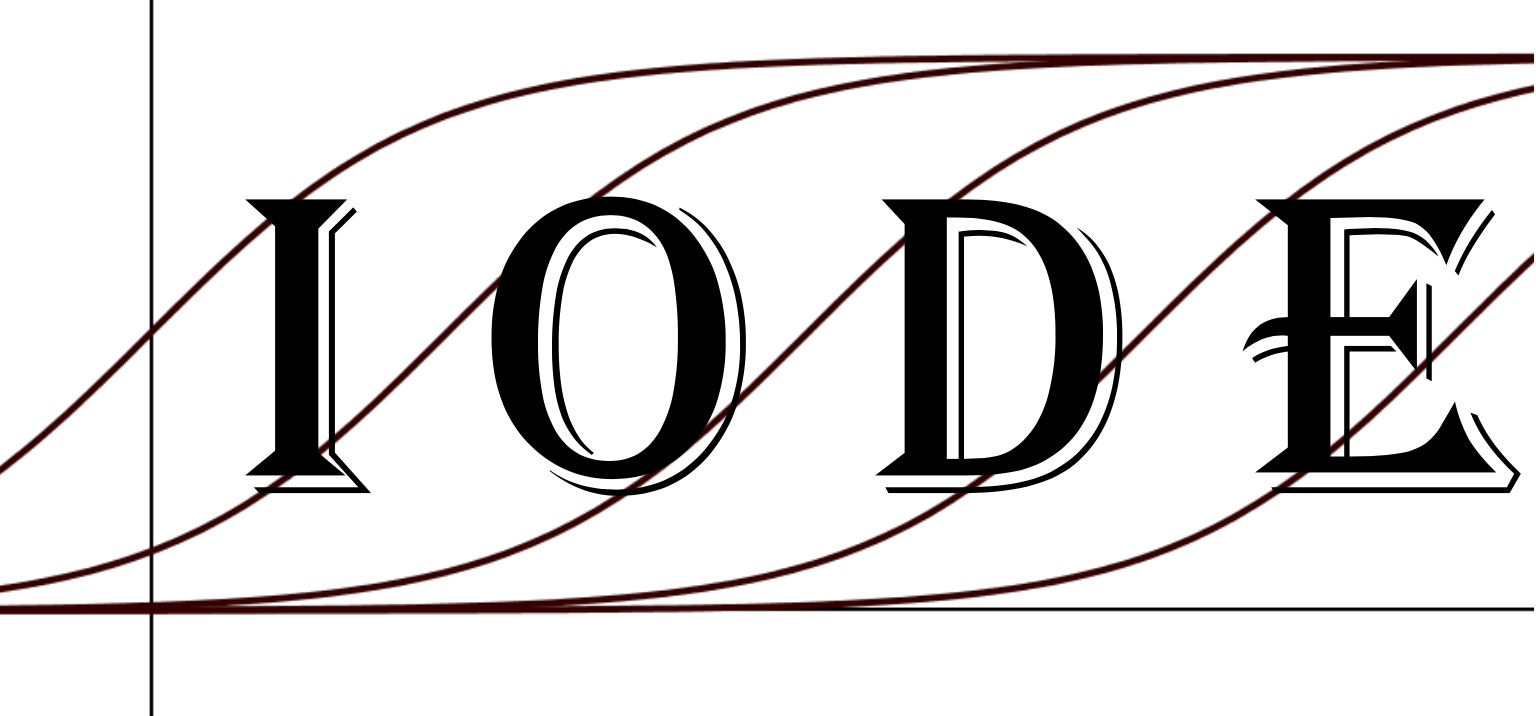
\includegraphics[width=1.25cm]{IODE-logo.png}}
\rfoot{\mypage}
\lfoot{}
\cfoot{}
\fancypagestyle{firstfooter}{\footskip = 50pt}
\renewcommand{\footrulewidth}{.4pt}
%%%%%%%%%%%%%%%%%%%%%%%%%%%
\vspace*{-20pt} \thispagestyle{firstfooter}
\pagebegin{Phase Plane Equations}

Consider a system of two differential equations:

\begin{align*}
\frac{dx}{dt} &=f(x,y) \\
\frac{dy}{dt} &=g(x,y)
\end{align*}

Recall from the chain rule we have
\[ \frac{dy}{dx} \frac{dx}{dt} = \frac{dy}{dt}, \]
which gives
\[ \frac{dy}{dx} = \frac{ \frac{dy}{dt}}{\frac{dx}{dt}} = \frac{g(x,y)}{f(x,y)}.\]


\begin{enumerate}
\item Write and solve the corresponding phase plane equation for  the system
\begin{align*}
\frac{dx}{dt} &=7y \\
\frac{dy}{dt} &=-2x
\end{align*}

\vfill

\item Make a sketch of several solutions in the phase plane, include arrows to indicate how solutions behave with respect to time.

\vfill

\end{enumerate}

\clearpage

\pagebegin{Equilibrium Solutions}

A point $(x_0,y_0)$ is called an \textbf{equilibrium} (or critical point) of the system 
\begin{align*}
\frac{dx}{dt} &=f(x,y) \\
\frac{dy}{dt} &=g(x,y)
\end{align*}
if both $f(x_0,y_0)=0$ and $g(x_0,y_0)=0$.

\bigskip

The corresponding solution $(x(t),y(t)) = (x_0,y_0)$ is called an \textbf{equilibrium solution}.

%\bigskip

%For example the system
%\begin{align*}
%\frac{dx}{dt} &=7y \\
%\frac{dy}{dt} &=-2x
%\end{align*}
%has one equilibrium $(x(t),y(t))=(0,0)$.

\begin{enumerate}[resume]
\ii Find the equilibrium to the system.
\bb
\ii $\dsty \begin{array}{l}
\frac{dx}{dt} =2x-y+8 \\
\frac{dy}{dt} =3x+6
\end{array}$
\vfill

\ii $\dsty \begin{array}{l}
\frac{dx}{dt} =y^2-xy \\
\frac{dy}{dt} =2xy-4
\end{array}$
\ee

\vfill

\pagebreak

\ii Find the equilibrium. Then find and solve the phase plane equation.
\bb
\ii $\dsty \begin{array}{l}
\frac{dx}{dt} =6x \\
\frac{dy}{dt} =3y
\end{array}$

\vfill

\ii $\dsty \begin{array}{l}
\frac{dx}{dt} =4-4y \\
\frac{dy}{dt} =-4x
\end{array}$


\vfill

\clearpage

\ii $\dsty \begin{array}{l}
\frac{dx}{dt} =2y^2-y \\
\frac{dy}{dt} =x^2y
\end{array}$

\vfill

\ee
\ee

\clearpage

%%%%%%%%%%%%%%%%%%%%%%%%%%%%%%%%%%%%%%%%%
\pagebegin{Homework Set 12}

\begin{enumerate}
\item Consider the system from questions \ref{12problem3}-\ref{12problem7} from Unit 12. What is the smallest value of $b$ for which we get solutions that, when viewed in the position-velocity plane, lie along a straight line? Algebraically support your conclusion. \label{12HWproblem1}

\item Straight line Solutions for Systems of the Form 
\begin{align*}
\frac{dx}{dt}&=ax+by\\
\frac{dy}{dt}&=cx+dy
\end{align*}
Systems of equations of the form above are a special type of \textbf{linear system}. Linear systems model important applications, such as the spring mass system. Moreover, it is possible to find the general solution for any such linear system. For each of the system of differential equations below, address the following questions: \label{12HWproblem2}
\begin{itemize}

\item	How many equilibrium solutions are there are and what are they?

\item	Are there solutions that, when viewed in the phase plane (i.e., the $ x-y$ plane), lie along a straight line? If so, algebraically figure out the exact slope of the straight line(s). 

\item	For those systems that do have solutions that, when viewed in the phase plane, lie along a straight line, figure out the exact $x(t)$ and $y(t)$ equations for any solution with initial condition on the straight line(s). 

\item	For those systems that have straight line solutions, write down the general solution.

\item	How would you classify the equilibrium solution? Create terms if needed to classify any new types of equilibrium solutions and explain the meaning of your terms.

\item	For those systems of differential equations that do have solutions that, when viewed in the phase plane, lie along straight lines, what do these straight lines look like in 3D? Provide your best 3D sketch.

\end{itemize}

\begin{enumerate*}
\item $\displaystyle\begin{aligned} \frac{dx}{dt}&=-3x+2y\\
		\frac{dy}{dt}&=6x+y \end{aligned}$ \hspace{.15in}
\item $\displaystyle\begin{aligned} \frac{dx}{dt}&=x+y\\
		\frac{dy}{dt}&=-x+y \end{aligned}$ \hspace{.15in}
\item $\displaystyle\begin{aligned} \frac{dx}{dt}&=-2x-2y\\
		\frac{dy}{dt}&=-x-3y \end{aligned}$ \hspace{.15in}
\item $\displaystyle\begin{aligned} \frac{dx}{dt}&=2x+2y\\
		\frac{dy}{dt}&=x+3y \end{aligned}$
\end{enumerate*}

\clearpage

\item You figured out from our analysis on the previous problems, sometimes there are solutions in the phase plane that lie along a straight line headed directly towards or away from the equilibrium solution at the origin and sometimes there are not. \label{12HWproblem3}

\begin{enumerate}
\item	Explain in words how you figure out whether there are any straight line solutions in the phase plane and if so, what the slopes of this line or lines are. Demonstrate how your approach works in general for linear systems of the form \label{12HWproblem3parta}
\begin{align*}
\frac{dx}{dt}&=ax+by\\
\frac{dy}{dt}&=cx+dy
\end{align*}

\item	Explain in words how you figure out the $x(t)$ and $y(t)$ equations for any and all straight line solutions in the phase plane. Demonstrate how your approach works in general for linear systems of the form \label{12HWproblem3partb} 
\begin{align*}
\frac{dx}{dt}&=ax+by\\
\frac{dy}{dt}&=cx+dy
\end{align*}

\item	Explain in words why having two different straight line solutions is useful for finding the $x(t)$ and $y(t)$ equations for any initial condition. \label{12HWproblem3partc}
\end{enumerate}

\clearpage

\item	Below is a vector field for the system of differential equations:
\begin{align*}
\frac{dx}{dt}&=2x+3y\\
\frac{dy}{dt}&=-4y
\end{align*}
Straight line solutions lie along the line $y = 0$ (with positive exponent in the $x(t)$ and $y(t)$ equations) and along the line $y = -2x$ (with negative exponent in the $x(t)$ and $y(t)$ equations).
\begin{center}
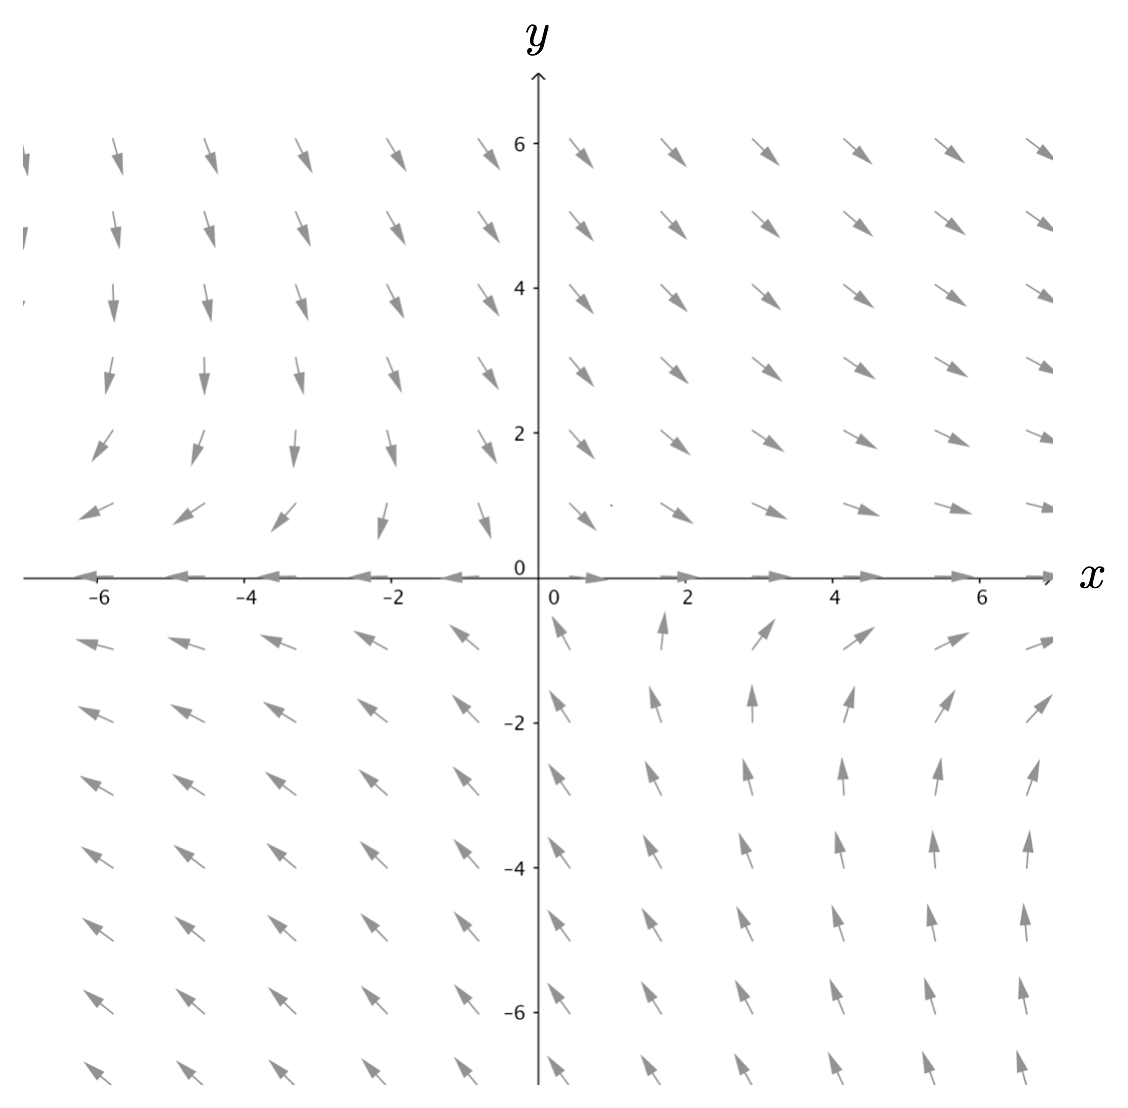
\includegraphics[width=4in]{12/12HWVectorField.png}
\end{center}
\begin{enumerate}
\item	Consider two different initial conditions, one at the point (1, 0) and one at the point (3, 0). Determine, with reasons, what happens to the graphs of the two solutions with these initial conditions as time progresses.\label{12HWproblem4parta} 
\item	Repeat problem \ref{12HWproblem4parta} for the initial conditions (-1, 2) and (-3, 6).\label{12HWproblem4partb}
\vfill

\end{enumerate}

\clearpage

\item	Find a value or a range of values for the parameter $n$ between -4 and 4 (including non-integer values) in the system of differential equations \label{12HWproblem5}
\begin{align*}
\frac{dx}{dt}&= -3x+ny\\ \frac{dy}{dt}&= 6x+y
\end{align*}  
so that when you view solutions in the $x$-$y$ plane there are
\begin{enumerate}
\item exactly two different straight line solutions \label{12HWproblem5parta}
\item	no straight line solutions \label{12HWproblem5partb}
\item	exactly one straight line solution \label{12HWproblem5partc}
\item	an infinite number of equilibrium solutions and an infinite number of straight line solutions \label{12HWproblem5partd}
\end{enumerate}

\item	Consider the following system of differential equations: \label{12HWproblem6}
\begin{align*}
\frac{dx}{dt}&= 2x \\ \frac{dy}{dt}&= 2y
\end{align*}  
\begin{enumerate}
\item Without using technology, sketch many different solutions in the phase plane. Explain your reasoning.  \label{12HWproblem6parta}
\item	Unlike other systems of differential equations that we have been studying, this system can be solved using techniques from our study of 1-dimensional systems.  What makes this system different?  \label{12HWproblem6partb}
\item	Find the general solution in two ways, one using separation of variables and the other using straight line techniques. \label{12HWproblem6partc}
\item	Explain how the general solution can help you make sense of the solution graphs in the phase plane.  \label{12HWproblem6partd}
\end{enumerate}

\item Without using technology, sketch many different solutions in the phase plane for the following system of differential equations. Explain your reasoning. [\textit{Hint}: how many equilibrium solutions are there?] \label{12HWproblem7}

\begin{align*}
\frac{dx}{dt}&= -3x-\frac{1}{2}y \\ \frac{dy}{dt}&= 6x+y
\end{align*}

\clearpage

\item \textbf{A Swaying Skyscraper}: The following system of rate of change equations is a model for helping us make predictions about the motion of a tall building.
\begin{align*}
\frac{dx}{dt}&= y \\
\frac{dy}{dt}&= -x-y+x^3
\end{align*}
In this simplified system of rate of change equations, $x$ stands for the amount of displacement of the building from the vertical position at any time $t$ and $y$ stands for the horizontal velocity of the building at any time $t$. Use the GeoGebra Vector Field applet, \href{https://ggbm.at/kkNXUVds}{\underline{https://ggbm.at/kkNXUVds}}, as a tool to explore solutions as viewed in the $xy$-plane (i.e., the phase plane). \label{12HWproblem8}

\vspace{-.5in}\hspace{-.6in}
\includegraphics[width=0.5in]{12/12VectorFieldQR.png}

\begin{enumerate}
\item Determine all equilibrium solutions and explain the meaning of each one in terms of the swaying skyscraper. Create any terms needed to classify new types of equilibrium solutions and briefly explain your reasons or imagery behind your choice of terms. \label{12HWproblem8parta}
 
\item Provide a sketch of several representative curves in the phase plane and give an interpretation for the motion of the building for the different types of curves (e.g., does the building remain standing? If so, for what initial conditions? For what range of initial conditions is a disaster predicted?) \label{12HWproblem8partb}
\end{enumerate}

\end{enumerate}


